\documentclass[tikz]{standalone}
\usepackage{amsmath,amssymb,multirow}
\usetikzlibrary{shapes.misc, positioning,automata,arrows,calc,fit}
\tikzset{VertexStyle/.style = {draw,circle,thick,
		minimum size=1cm,
		font=\Large\bfseries},thick} 
\usepackage{booktabs}
\begin{document}
	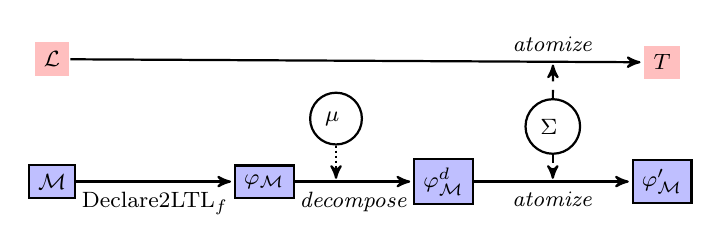
\begin{tikzpicture}[->,>=stealth',shorten >=1pt,thick,initial text=$ $,align=center,node distance=5mm,font=\footnotesize]
	\thickmuskip=0mu
	%% Input
	\node (Clause)  [fill=blue!25,shape=rectangle,draw=black] 
	{$\mathcal{M}$};
	
	%% Straightforward translation
	%\node (LTLf1) 
	%				[right=2cm of Clause,fill=blue!25,text width=3cm,rounded corners=.3cm,draw=black] 
	%				{$\square(\texttt{A}\Rightarrow \lozenge(\texttt{B}\wedge \texttt{B}.x>0))$\\
	%				 $\lozenge(\texttt{B}\wedge \texttt{B}.x>3\wedge \texttt{B}.y=0)$};
	
	%% Conversion to NNF				
	\node (LTLf2) 	[right=2cm of Clause,fill=blue!25,shape=rectangle,draw=black] 
	{$\varphi_{\mathcal{M}}$};
	\draw[->] (Clause) -- (LTLf2) node[midway,below] {Declare2LTL$_f$} ;
	%\draw[->] (LTLf1) --  (LTLf2) node[midway,above] {\textit{nnf}};
	
	%% Data predicates decomposition
	\node (LTLf3) 	[right=1.5cm of LTLf2,fill=blue!25,shape=rectangle,draw=black] 
	{$\varphi_{\mathcal{M}}^d$};
	\draw[->] (LTLf2) --  (LTLf3) node[midway,below] {\textit{decompose}};
	
	\node (tab1) [ shape=circle,draw] at ($(LTLf2)!0.4!(LTLf3)+(0,.8)$) {
$\mu$
	};
	\draw[->,densely dotted] (tab1) -- ($(LTLf2)!0.4!(LTLf3)$);
	
	\node (LTLf4) 	[right=2cm of LTLf3,fill=blue!25,shape=rectangle,draw=black] 
	{$\varphi_{\mathcal{M}}'$};
	
	\node (Traces) [fill=red!25,above=1.1cm of Clause] 
	{$\mathcal{L}$};
	
	\node (CTraces) [fill=red!25,above=1cm of LTLf4] 
	{{$T$}};
	
	%\node[state,initial] (SA) at ($(LTLf4)-(1.3,3.5)$) {$s_1$};
	%\path (SA) edge[loop] node[midway,above] (W1) {$\Sigma\backslash\{p_1,p_3\}$} (SA);
	%\node[state,accepting,right =2cm of SA] (ST) {$s_2$};
	%\path (ST) edge[loop] node[midway,above] (W2) {$\Sigma\backslash\{p_3\}$} (ST);
	%\draw[->] (SA) -- (ST) node[midway,above] {$\{p_1\}$};
	%\node[state] (bot) at ($(SA)!0.5!(ST)-(0,2.5)$) {$\bot$};
	%\draw[->] (SA) -- (bot) node[midway,below,sloped] {$\{p_3\} $} ;
	%\draw[->] (ST) -- (bot) node[midway,below,sloped] {$\{p_3 \}$} ;
	%\draw (bot) to [in=225,out=315,looseness=8] node[midway,above] (W3) {$\Sigma$} (bot);
	%\node[draw=black,fit=(SA) (ST) (W1) (W2) (bot) (W3)] (NFA) {};
	
	
	
	\draw[->] (LTLf3) -- (LTLf4) node[midway,below]  {\textit{atomize}};
	
	
	
	
	\draw[->] (Traces) -- (CTraces);
	\node (tab2) [shape=circle,draw] at ($(LTLf4)!0.5!(LTLf3)+(0,.7)$) {
$\Sigma$
	};
	
	\draw[->,dashed] (tab2) -- ($(Traces)!(tab2.north)!(CTraces)$) node [above] {\textit{atomize}};
	\draw[->,dashed] (tab2) -- ($(LTLf3)!0.5!(LTLf4)$);
	
	%
	%\draw[->] (LTLf4) -- (NFA) node[midway,left] {LTL$_f$2DFA};
	\end{tikzpicture}
\end{document}